% Esta plantilla ha sido diseñada por Daniel del Río Velilla, profesor en la Escuela de Aeronáutica y del Espacio, UPM.

\documentclass[11pt,a4paper,titlepage,twoside]{report}

%   ---   DEFINICION DEL TRABAJO   ---   %

\newcommand{\Project}{Plantillas de \LaTeX}
\newcommand{\ProjectTitle}{Plantilla de \LaTeX\, para tesis}
\newcommand{\ProjectSubject}{Grado de Ingeniería Aeroespacial}
\newcommand{\ProjectAutor}{ Alumno 1 \\
                            & Alumno 2}
\newcommand{\ProjectTutor}{ Tutor 1 \\
                            & Tutor 2}
\newcommand{\ProjectLocation}{Madrid}
\newcommand{\ProjectDate}{19 de septiembre de 2022}
% Descomentar si se tiene un repositorio del trabajo
% \newcommand{\ProjectGitHub}{url}



%   ---   INCLUIR ARCHIVOS DE CONFIGURACION   ---   %

\usepackage[utf8]{inputenc}         % Permite escribir códigos especiales

% AJUSTES DEL IDIOMA
\usepackage[spanish]{babel}
\decimalpoint
\renewcommand{\spanishtablename}{Tabla}
\addto\extrasenglish{
    \renewcommand{\subsubsectionautorefname}{Section}
    \renewcommand{\subsectionautorefname}{Section}
    \renewcommand{\sectionautorefname}{Section}
}
\usepackage[title]{appendix}
\renewcommand{\appendixname}{Anexos}
\renewcommand{\appendixtocname}{Anexos}
\renewcommand{\appendixpagename}{Anexos}


% GEOMETRIA
\usepackage[paper=A4]{typearea}
\usepackage[includemp,
            top=2 cm,
            left = 1.2 cm, 
            right = 1.2 cm,
            bottom=2 cm,
            headsep = 3.5 cm,
            marginparwidth=2 cm,
            marginparsep=0.4 cm]{geometry}


% INDENTACION
\usepackage{indentfirst}
\setlength{\parskip}{5pt}       
\setlength{\parindent}{0pt}


% ESPACIADO
\usepackage{setspace}
\spacing{1.2}
\let\ph\mlplaceholder % shorter macro


% GENERAR PDF/A y otras cosas del pdf
\usepackage[a-1b]{pdfx}
\usepackage[pdftex]{graphicx}
    \graphicspath{
      {./Figures/Portada_HF/}
      {./Figures/01/}
      {./Figures/02/}
      {./Figures/03/}
      {./Figures/04/}
      {./Figures/05/}
      {./Figures/06/}
      {./Figures/A_01/}
      {./Figures/A_02/}
    }
\usepackage{pdfpages}               % Incluir PDF diferente tamaño


% URLS Y LINKS
\hypersetup{hidelinks}    % Hide borders links
\usepackage{url}
\Urlmuskip=0mu plus 1mu


% EXPRESIONES MATEMATICAS Y SÍMBOLOS
\usepackage{textcomp}               % Symbols in text
\usepackage{amsmath}
\usepackage{amssymb}
\usepackage{mathtools}
\usepackage[T1]{fontenc}
\usepackage{mathtools}
\usepackage{mathrsfs}
\usepackage{derivative}
\usepackage{amsmath,amssymb}
\usepackage{float}
\DeclareMathOperator{\Tr}{Tr}
\usepackage{bigints}
\usepackage{gensymb}    % Para hacer los circulitos de grados
\usepackage{eurosym}
\usepackage{fontawesome}


% INCLUIR CÓDIGO EN EL DOCUMENTO
\usepackage{listings}
\renewcommand{\lstlistingname}{Listado}		% Para que las listas sean es español
\usepackage[framed,numbered,autolinebreaks,useliterate]{mcode}      % MATLAB CODE
% \lstset{
%     inputencoding=utf8,
%     literate={Á}{{\'A}}1 {á}{{\'a}}1 {É}{{\'E}}1 {é}{{\'e}}1 {Í}{{\'I}}1 {í}{{\'i}}1 {Ó}{{\'O}}1 {ó}{{\'o}}1 {Ú}{{\'U}}1 {ú}{{\'u}}1 
%     }

%\lstset{
%  basicstyle         = \mlttfamily,
%  escapechar         = ",
%}
%\usepackage[numbered]{matlab-prettifier}


% ACRONIMOS
% https://tex.stackexchange.com/questions/25520/how-can-i-use-the-latex-acronym-package-and-optionally-create-an-acronym-list-i
% https://sourceforge.net/p/texstudio/discussion/907839/thread/7ced058c/  -> SI NO APARECEN LOS ACRONIMOS
\usepackage[acronym,smallcaps]{glossaries}		% ,nonumberlist
% \loadglsentries[\acronymtype]{./Tex_Files/acronyms.tex}
\makeglossaries
%\usepackage{nomencl}
%\makenomenclature
%\usepackage{etoolbox}
%\renewcommand\nomgroup[1]{%
%  \item[\bfseries
%  \ifstrequal{#1}{P}{Propiedades físicas}{%
%  \ifstrequal{#1}{S}{Señales ópticas}{%
%  \ifstrequal{#1}{F}{Fibra óptica}{%
%  \ifstrequal{#1}{C}{Material compuesto}{}}}}%
% ]}


% BIBLIOGRAFÍA
%\usepackage{biblatex}
%\addbibresource{references.bib}
%\setlength\parindent{0pt}


% DISEÑO DE TABLAS Y FIGURAS 
% \usepackage{subfigure}
% \usepackage{subfloat}
\usepackage{caption}
\usepackage{subcaption}		% https://tex.stackexchange.com/questions/295456/texstudio-beginsubfigure-unrecognized-command
\usepackage{svg}
\usepackage{import}
\usepackage{longtable}
\usepackage{multirow}
\usepackage{multicol}
\usepackage{threeparttable}
\usepackage{booktabs}
\usepackage{tabu}
\usepackage{bigstrut}
\usepackage{tabularx}
    \makeatletter
    \def\hlinewd#1{%
    \noalign{\ifnum0=`}\fi\hrule \@height #1 \futurelet
    \reserved@a\@xhline}
    \makeatother
\usepackage{placeins}  %para poder poner Floatbarrier


% ENUMERACIONES
\usepackage{enumerate}
\usepackage{enumitem}  % Selecionar la forma del item


% NOTAS PIE DE PAGINA
\usepackage[colorinlistoftodos]{todonotes}  % TO DO
\newcommand\blfootnote[1]{%
  \begingroup
  \renewcommand\thefootnote{}\footnote{#1}%
  \addtocounter{footnote}{-1}%
  \endgroup
}


% DEFINICIÓN DE COLORES 
\usepackage{xcolor}
\usepackage{colortbl}


% COMANDOS
\providecommand\phantomsection{}    % Para añadir phantomsections al indice


% LANDSCAPE
\usepackage{pdflscape}
\usepackage{everypage}
\usepackage{lipsum}
% Landscape configuration
\newcommand{\Lpagenumber}{\ifdim\textwidth=\linewidth\else\bgroup
  \dimendef\margin=0 %use \margin instead of \dimen0
  \ifodd\value{page}\margin=\oddsidemargin
  \else\margin=\evensidemargin
  \fi
  \raisebox{\dimexpr -\topmargin-\headheight-\headsep-0.5\linewidth}[0pt][0pt]{%
    \rlap{\hspace{\dimexpr \margin+\textheight+\footskip}}}%
\egroup\fi}
\AddEverypageHook{\Lpagenumber}%
% Code
%\begin{landscape}
% Text
%\end{landscape}


% MISCELANEO
\usepackage{cite}
\usepackage{csquotes} % Cita en el texto
\usepackage{comment} % Comentar en bloque
\usepackage{lastpage} % Citar la última página
\usepackage{relsize} % Tamaños relativos
\usepackage{bm} % Para poner negrita math tablas
\usepackage{printlen}
\usepackage{afterpage}	% añadir algo despues de una pagina
\newacronym{mc}{MC}{Materiales Compuestos}
\newacronym{cfrp}{CFRP}{Carbon Fiber Reinforced Polymer}
\newacronym{udpp}{UDPP}{Unidirectional Prepeg}
\newacronym{fr}{FR}{Filament Ripper}
\newacronym{rrf}{RRF}{RepRap Firmware}
\newacronym{dwc}{DWC}{Duet Web Control}
\newacronym{sbc}{SBC}{Single Board Computer}
\newacronym{rsp}{RSP4}{Raspberry Pi 4}
\newacronym{cad}{CAD}{Computer Aided Desing}
\newacronym{rpas}{RPAS}{Remotely Piloted Aircraft System}
\newacronym{ba}{BA}{Borde de ataque}
\newacronym{bs}{BS}{Borde de salida}
\newacronym{eop}{EoP}{Edge of Part}
\newacronym{eeop}{EEoP}{Engineering Edge of Part}
\newacronym{meop}{MEoP}{Manufacturing Edge of Part}
\newacronym{eom}{EoM}{Excess of Material}


% DISEÑO DE CABECERA Y PIE DE PÁGINA
\lstMakeShortInline"
\newlength{\myoddoffset}
\setlength{\myoddoffset}{\marginparwidth + \marginparsep + 0.5cm}
\usepackage{fancyhdr}
\fancyheadoffset[rh]{\myoddoffset}
\fancyfootoffset[rh]{\myoddoffset}

\pagestyle{fancy}
\fancyhf{}
\fancyhead[R]{ \hspace{2pt} \rightmark}
\lhead{
    
\includegraphics[width = 4.2cm]{upm_logo.png}
}
\rhead{
    \begin{Large}{\Project}\end{Large}
}
% \lfoot{} \cfoot{} \rfoot{\thepage}
\fancyfoot[RO]{\thepage}


\newgeometry{
    top=1.7in, 
    bottom=1.1in, 
    left = 2.5cm, 
    right = 2cm, 
    headsep = 2.5cm, 
    ignoremp
}
\fancyheadoffset[rh]{0pt}
\fancyfootoffset[rh]{0pt}

\fancypagestyle{plain}{		% Modificar el pagenumber en los capitulos
	\fancyhf{} 
	\fancyfoot[RO]{\thepage} % same placement as with page style "fancy"
	\renewcommand{\headrulewidth}{0pt}
	}
	


% % ABSTRACT
% \def\changemargin#1#2{\list{}{\rightmargin#2\leftmargin#1}\item[]}
% \let\endchangemargin=\endlist 
% \newcommand\summaryname{Abstract}
% \newenvironment{Abstract}%
%     {\small\begin{center}%
%     \bfseries{\summaryname} \end{center}}
\newcommand{\clearemptydoublepage}{
    \newpage{\pagestyle{empty}\cleardoublepage}
}

\newcommand\blankpage{%
    \null
    \thispagestyle{empty}%
    \addtocounter{page}{-1}%
    \newpage}



%   ---   COMIENZO DEL DOCUMENTO   ---   %

\begin{document}


%   ---   INCLUIR PORTADA   ---   %

\begin{titlepage}
	\begin{center}
		\vspace*{0in}
		\begin{figure}[htb]
			\centering
			
\includegraphics[width = 0.6\linewidth]{./Figures/Portada_HF/upm_logo.png}
		\end{figure}
		
		\vspace*{0.2in}
		\rule{\linewidth}{0.4mm}\\
		\vspace*{0.1in}
		\begin{huge}
			\textbf{\scshape{\ProjectTitle}} \\
		\end{huge}
		\vspace*{0.1in}
		\begin{large}
			\begin{normalsize}
				\scshape{\Project}\\
				\scshape{\ProjectSubject}
			\end{normalsize}
		\end{large} 
		\vspace*{0.2in}
		\rule{\linewidth}{0.4mm}\\
		\vspace*{0.6in}
		\begin{large}
			\begin{tabular}{c}
				\\
				\begin{tabular}{ l l }
					\textit{Autor}: & \ProjectAutor     \\
					                &                   \\
					\textit{Tutor}: & \ProjectTutor     \\
					                &                   \\
				\end{tabular}
				
				
			\end{tabular}
		\end{large}
		
		\vspace*{0.5in}
		\begin{large}
			\textsc{\ProjectLocation, \ProjectDate}
		\end{large}
	\end{center}
	
	% Repositorio: descomentar si se usa un repo
	% \begin{center}
		% \vspace*{\fill}\begin{LARGE}\faGithub\end{LARGE}\hspace{2mm}\url{\ProjectGitHub}
	% \end{center}
	
	\afterpage{\blankpage}      % Anadir unas pagina en blanco despues del titulo
	
\end{titlepage}




%   ---   INDICE Y LISTAS   ---   %

% Indice
\pagenumbering{gobble}
\tableofcontents
\newpage

% Numeracion en romano
\pagenumbering{roman}
\raggedbottom

% Figuras    
\addcontentsline{toc}{section}{\listfigurename}
\listoffigures
\cleardoublepage

% Tablas
\renewcommand{\listtablename}{Índice de tablas}
\addcontentsline{toc}{section}{\listtablename}
\listoftables
\cleardoublepage

% Acronyms  
\renewcommand{\acronymname}{Acrónimos}
\addcontentsline{toc}{section}{\acronymname}
\printglossary[type=\acronymtype]   % \printglossary[type=\acronymtype,style=long]
\cleardoublepage

% Numeracion en arabico
\setcounter{page}{0}
\pagenumbering{arabic}



%   ---   ARCHIVOS DEL DOCUMENTO   ---   %
% Es recomendable escribir el trabajo en documentos separados y luego importarlos al main.

\section{Seción} \label{s:section_01}

En este capítulo se muestran varios ejemplos.

\textbf{Negrita} \textit{cursiva}

Hacer una referencia, en este caso al \autoref{s:section_01}.

% ---   ---   --- %


\subsection{Subseccion}

\subsubsection{Citar referencias y acrónimos}

\cite{im78552}, \acrshort{mc}, \acrfull{mc}.

\subsubsection{Enumeraciones}

Enumeración.

\begin{enumerate}
	\item La impresora debe contar con un sistema de nivelación de la base de impresión.
	\item El sistema de extrusión de filamento debe asegurar que no se producirán inconsistencias durante los periodos largos de trabajo.
\end{enumerate}

Enumeración cambiando los items.

\begin{enumerate}[label= \textbf{R-\arabic*}]
	\item La impresora debe contar con un sistema de nivelación de la base de impresión.
	\item El sistema de extrusión de filamento debe asegurar que no se producirán inconsistencias durante los periodos largos de trabajo. \label{req:extrusion}
\end{enumerate}

Referenciar un item: \ref{req:extrusion}, \autoref{req:extrusion}.


Ejemplo de bulletpoints.


\begin{itemize}[label={\scriptsize\raisebox{0.5ex}{\textbullet}}]

	\item Perfilería de aluminio.

\end{itemize}



%   ---   ---   %

\subsubsection{Figuras}

Las figuras se pueden fijar en el texto con H, posicionarlas lo mejor posible con h!, arriba con t, etc.

\begin{figure}[H]
	\centering
	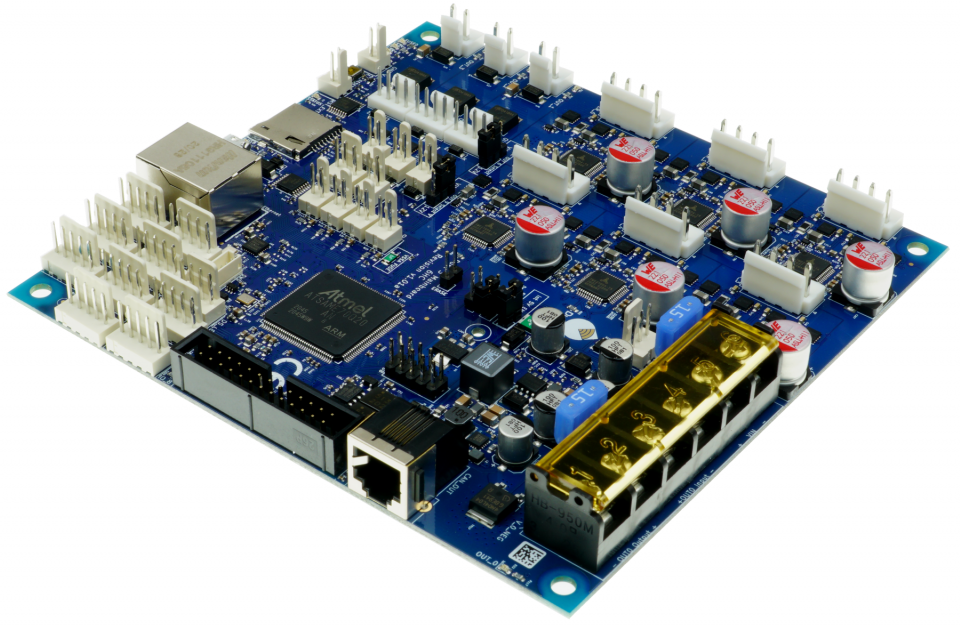
\includegraphics[width=100mm]{duet3}
	\caption{Motherboard Duet 3 6HC.}
	\label{fig:000_00}
\end{figure}

Subfiguras en paralelo.

\begin{figure}[H]
	\centering
	\subfloat[Vista frontal del montaje.\label{fig:mont1}]
	{
		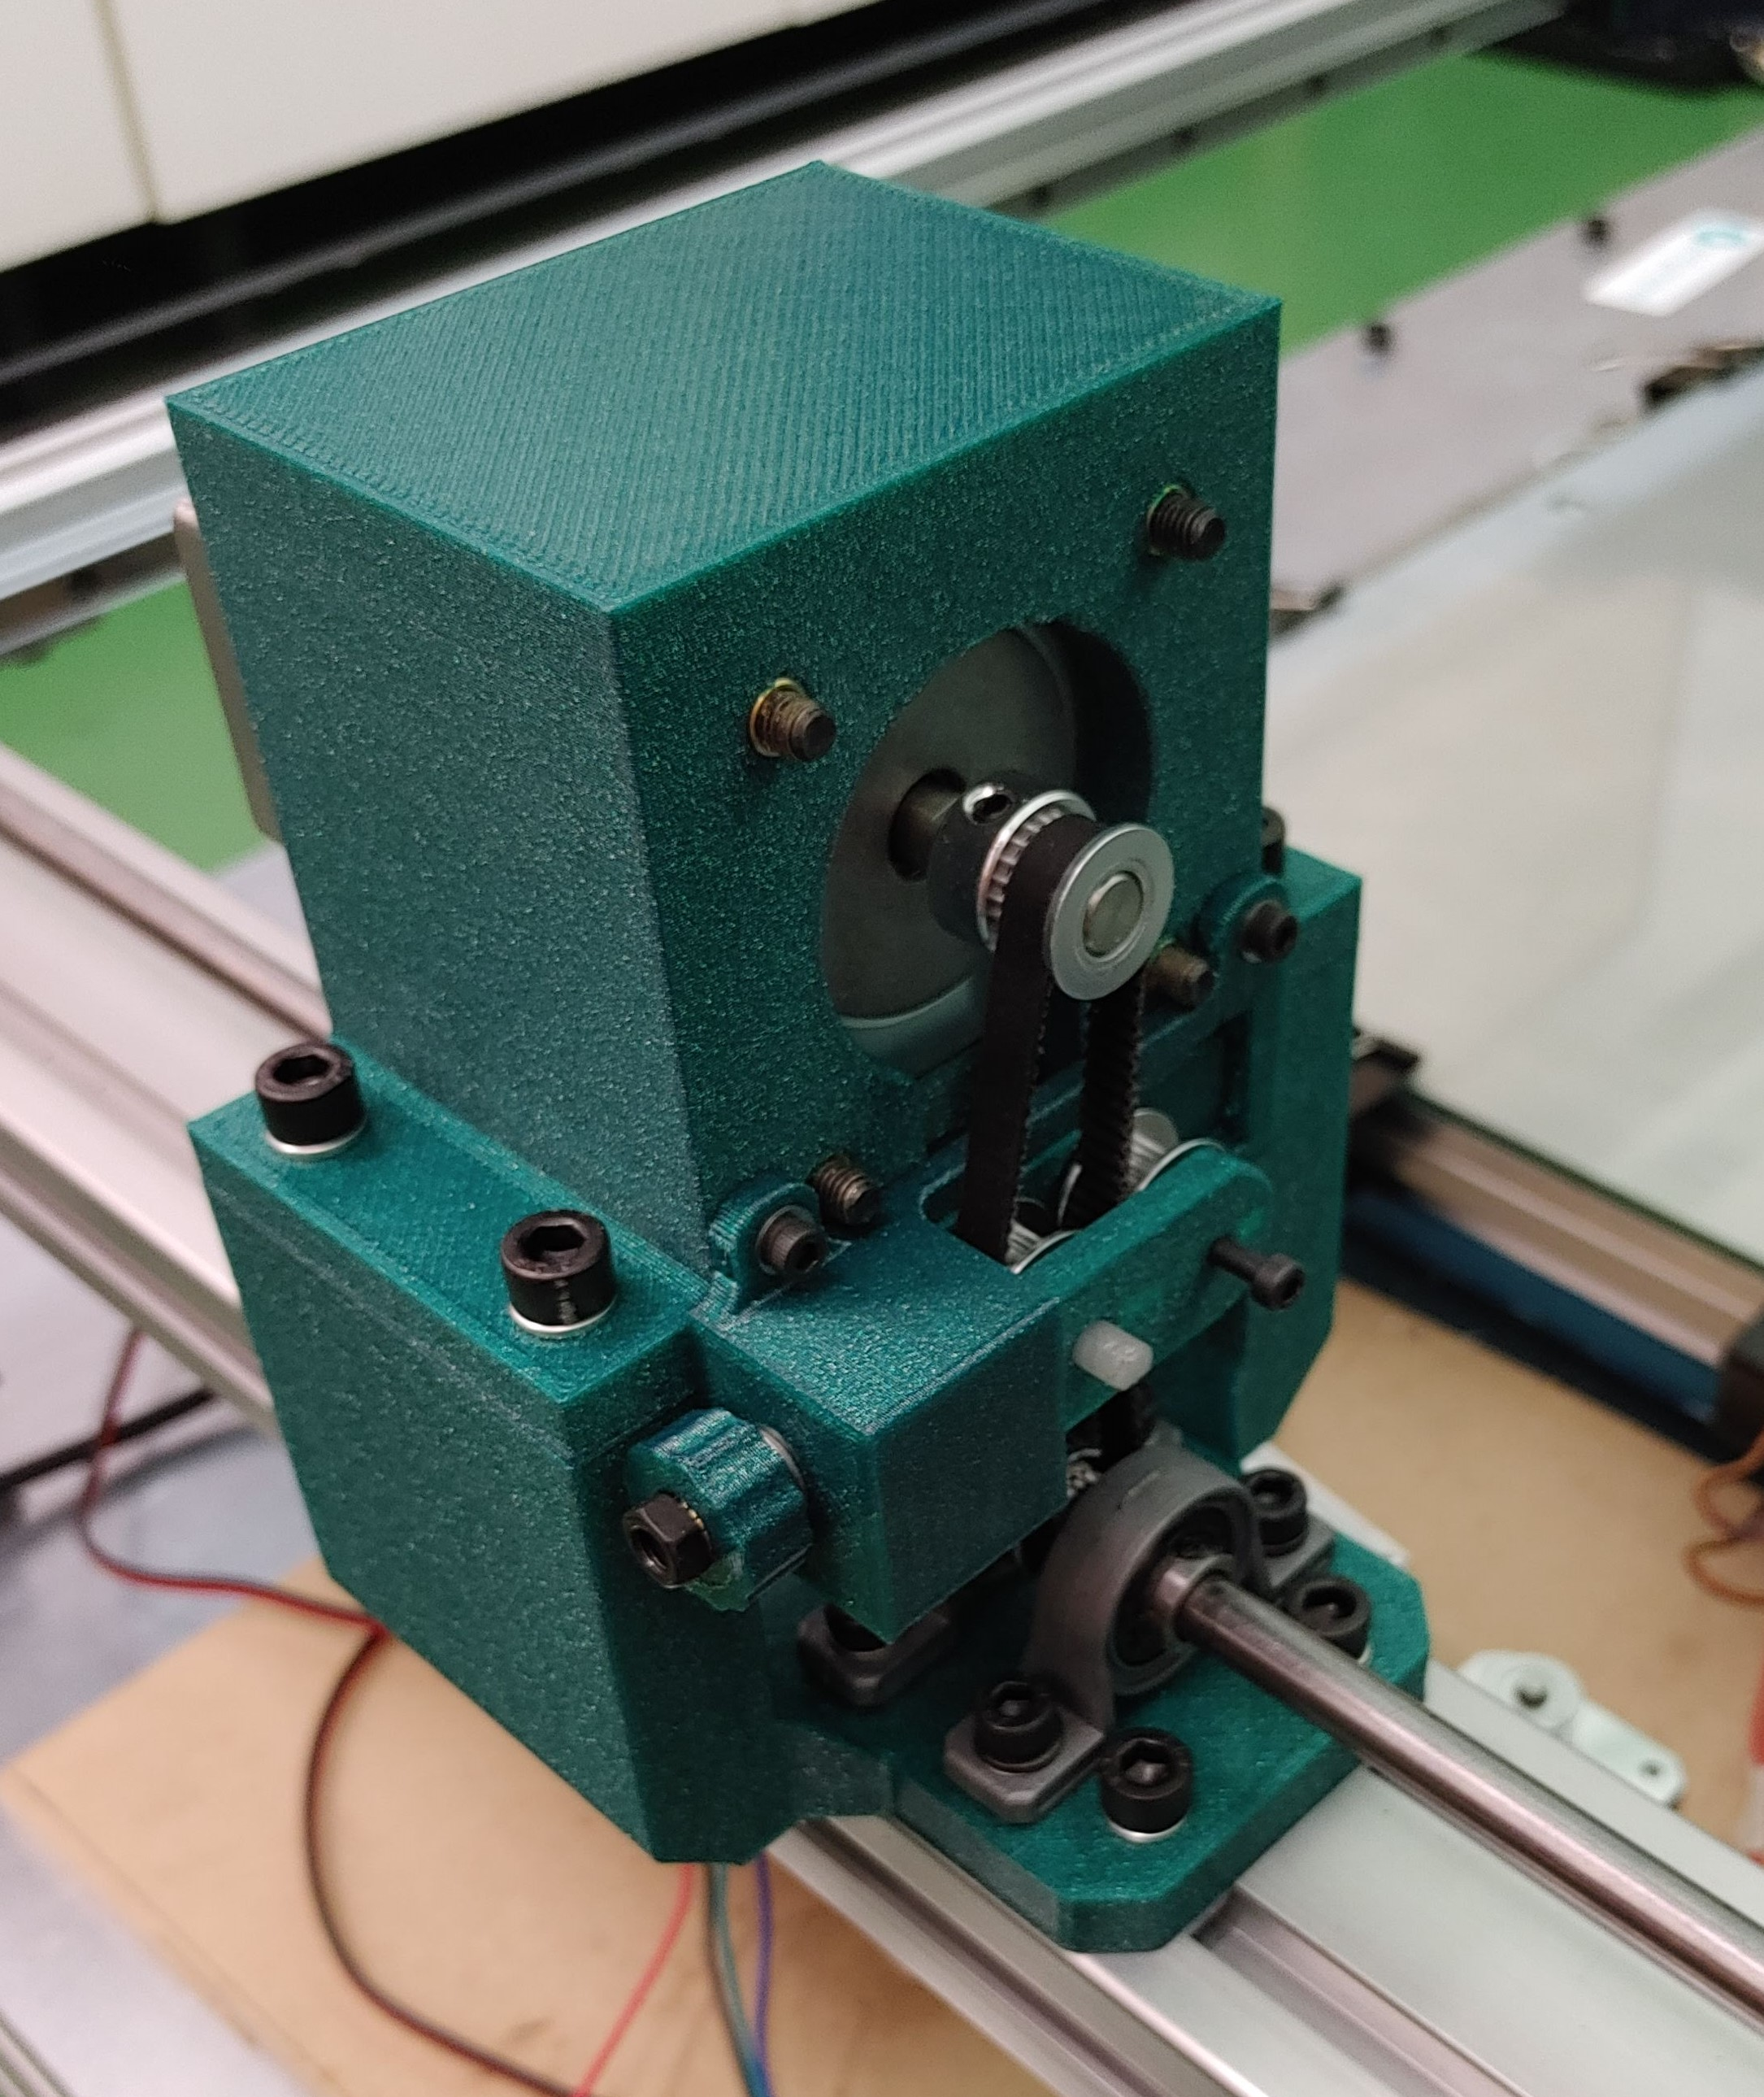
\includegraphics[width=50mm,angle=0]{Mont_01}
	}
	\hspace*{10mm}
	\subfloat[Vista trasera del montaje.\label{fig:mont2}]
	{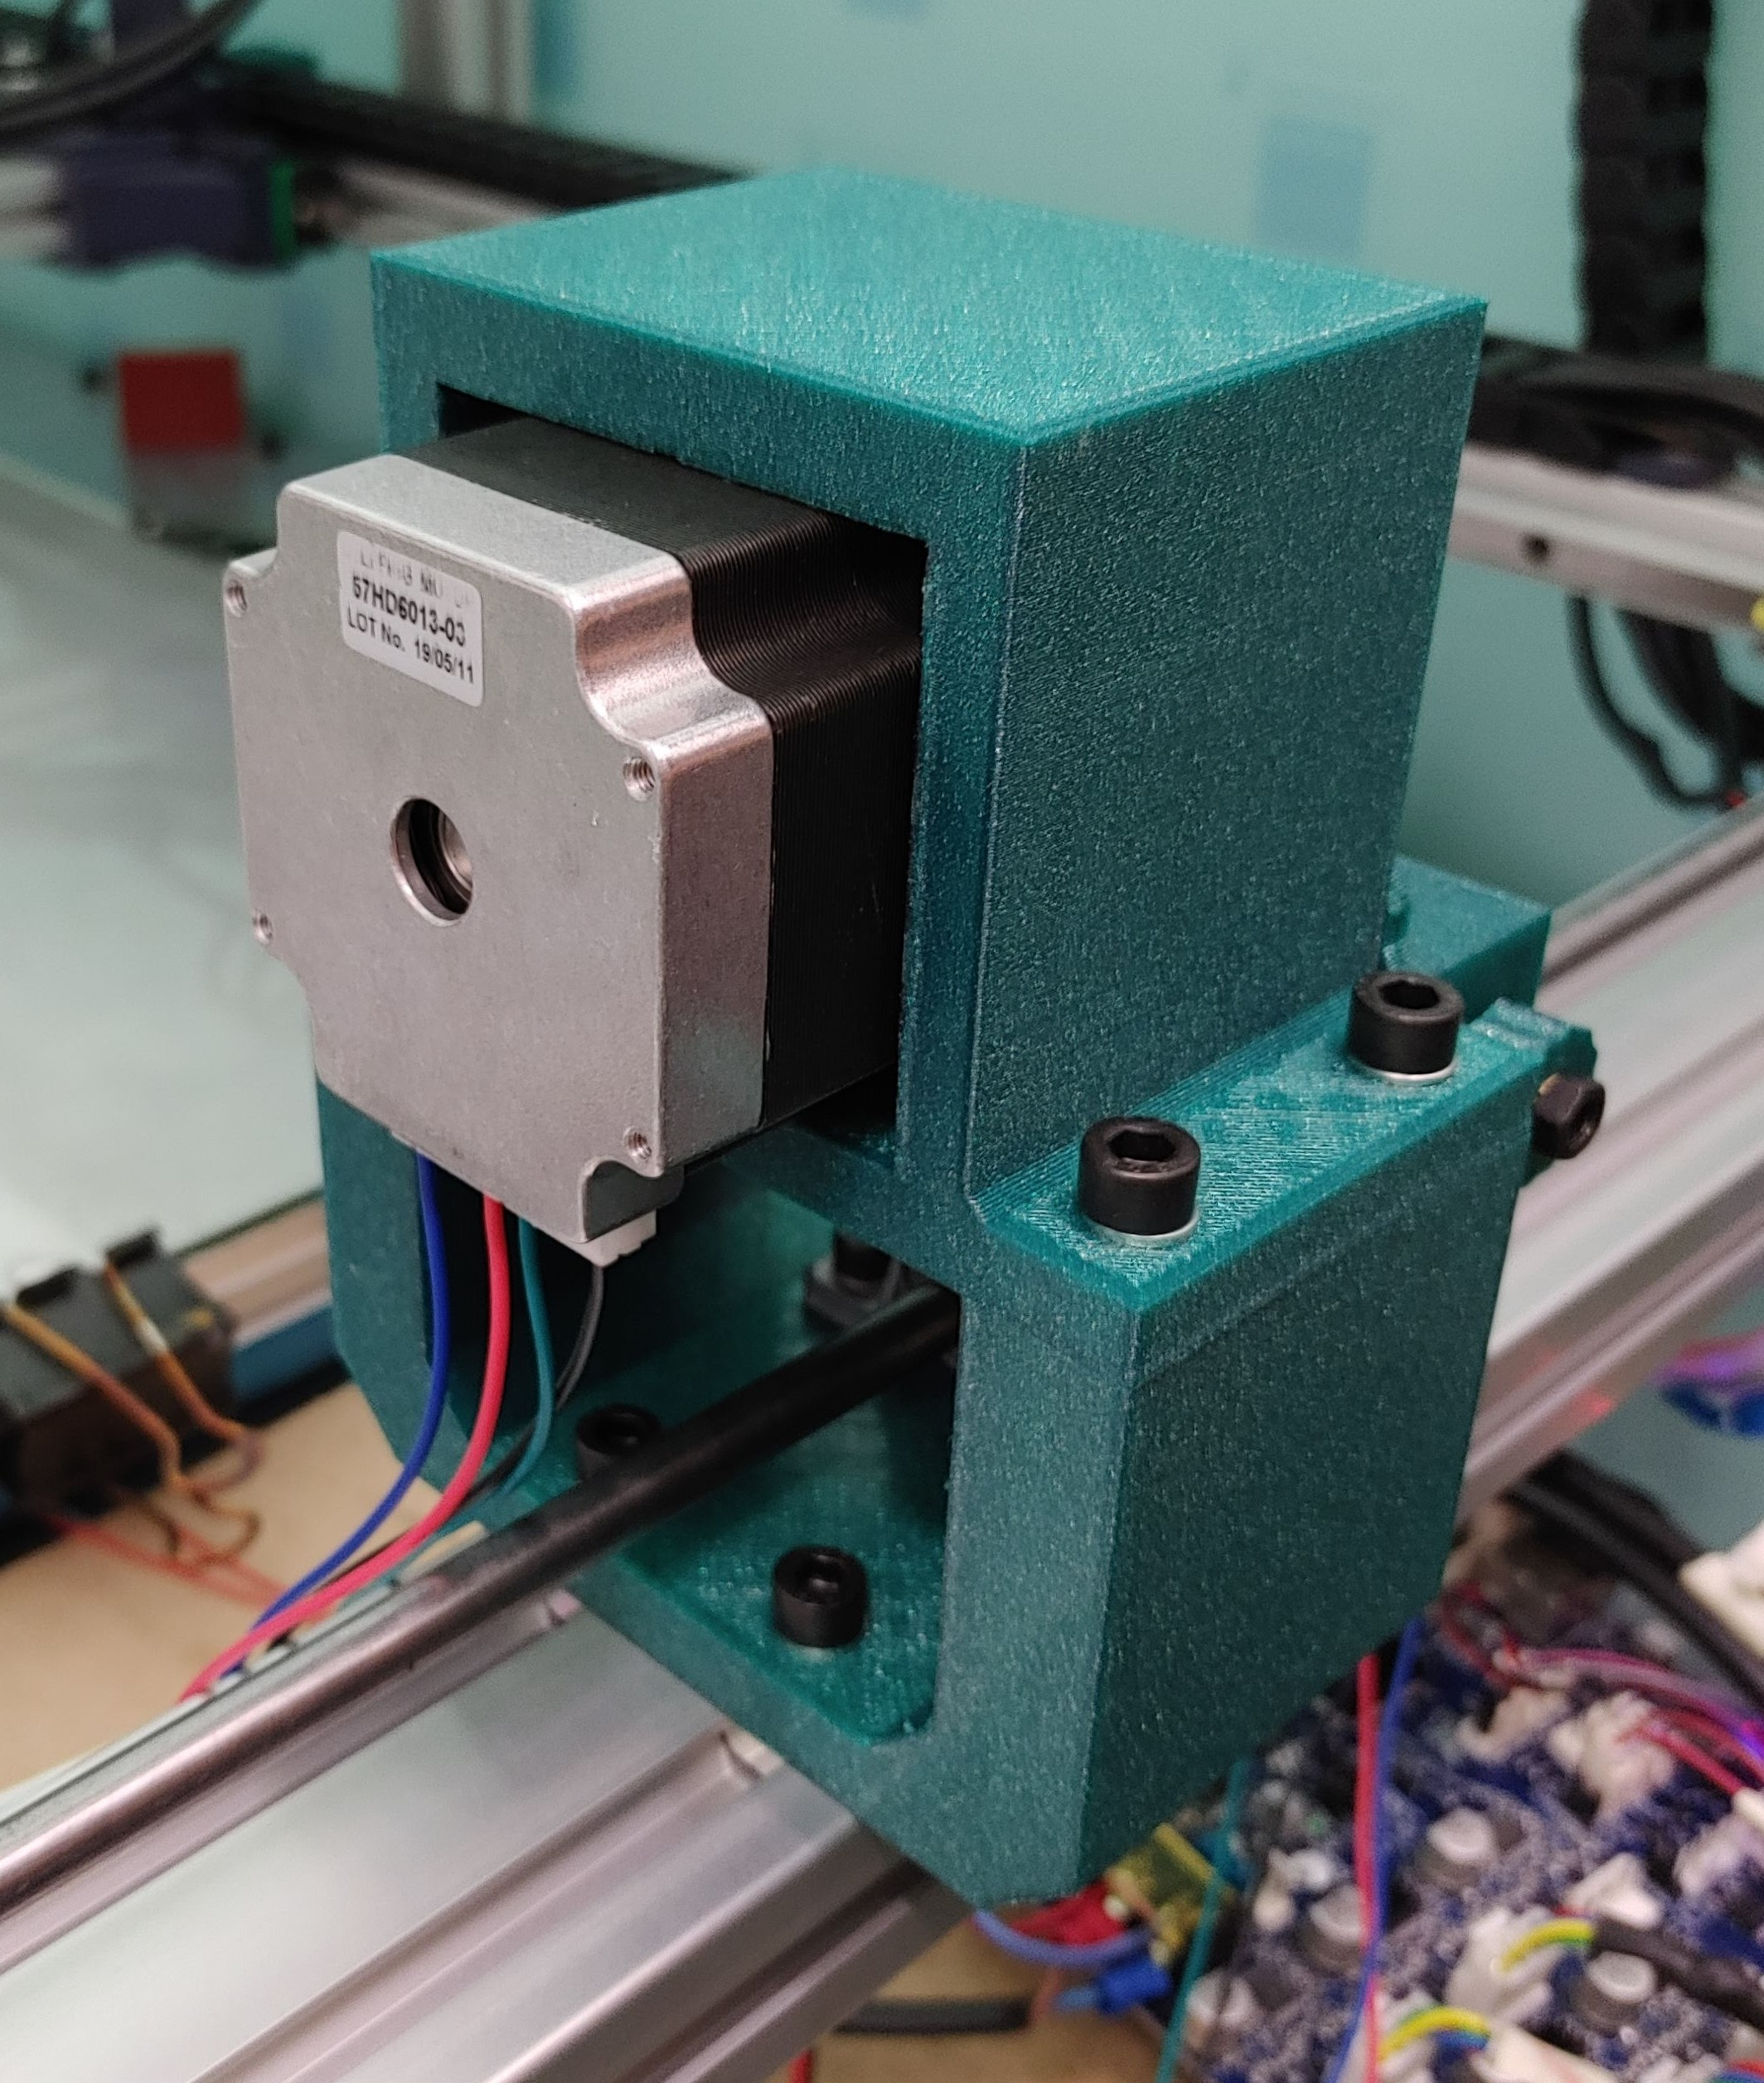
\includegraphics[width=50mm,angle=0]{Mont_02}
	}
	\caption{Montaje del sistema de transmisión del eje X}
	\label{fig:mont_nema}
\end{figure}


Ejemplo dos figuras en paralelo centradas verticalemtne.

\begin{figure}[H]
	\begin{minipage}{\textwidth}
		\centering
		\raisebox{-0.5\height}{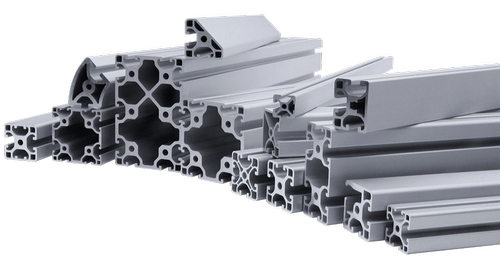
\includegraphics[width=0.4\textwidth]{Perfil_Aluminio}}
	\hspace*{.2in}
		\raisebox{-0.5\height}{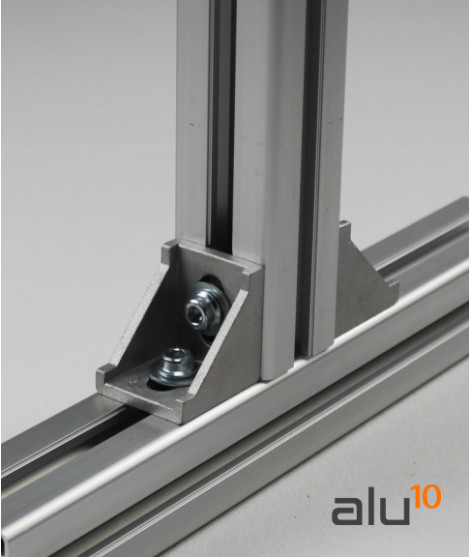
\includegraphics[width=0.25\textwidth]{Perfil_Aluminio_Union}
		}
	\end{minipage}
	\caption{Ejemplos de perfilería de aluminio.}
	\label{fig:perfileria_alumnio}
\end{figure}

Barrera que no pueden atravesar las figuras.
\FloatBarrier


%   ---   ---   %

\subsubsection{Ecuaciones}

Ejemplo de ecuación, \autoref{eq:velocidad}

\begin{equation}\label{eq:velocidad}
	l = \frac{\pi\cdot1.8}{180\cdot P}\cdot r = \frac{\pi\cdot1.8}{180\cdot16}\cdot 6 = 0.0117 \qquad [\mathrm{mm}].
\end{equation}



% ---   ---   --- %

\subsubsection{Tablas}

Ejemplo de tabla de grandes dimensiones e introducir una página apaisada. También se muestra como poner en negrita letras griegas, que a veces dan problemas.

\begin{landscape}
    \vspace*{\fill}
    \begin{table}[H]
    \centering
    \caption{Resultados del estudio paramétrico del modelo de localización (2 de 2).}
        \label{tab:Results_XY_2}
        \resizebox{23cm}{!} {
        {\renewcommand{\arraystretch}{1.2}
        
        
    \begin{tabular}{|r|r|r|r|l|l|l|l|l|l|l|l|l|}
    \hline
    \rowcolor[HTML]{C0C0C0} 
    \multicolumn{1}{|c|}{\cellcolor[HTML]{C0C0C0}} & 
    \multicolumn{3}{c|}{\cellcolor[HTML]{C0C0C0}\textbf{Parámetros}} & 
    \multicolumn{3}{c|}{\cellcolor[HTML]{C0C0C0}\textbf{Distancia}} & 
    \multicolumn{3}{c|}{\cellcolor[HTML]{C0C0C0}\textbf{X}} &
    \multicolumn{3}{c|}{\cellcolor[HTML]{C0C0C0}\textbf{Y}} 
    
    \\ \cline{2-13} 
    
    \rowcolor[HTML]{EFEFEF} 
    \multicolumn{1}{|c|}{\multirow{-2}{*}{\cellcolor[HTML]{C0C0C0}Id}} & 
    \multicolumn{1}{c|}{\cellcolor[HTML]{EFEFEF}\textbf{outFE}} & 
    \multicolumn{1}{c|}{\cellcolor[HTML]{EFEFEF}\textbf{compFE}} & 
    \multicolumn{1}{c|}{\cellcolor[HTML]{EFEFEF}\textbf{compReg}} & 
    \multicolumn{1}{c|}{\cellcolor[HTML]{EFEFEF}$\bm{\mu}$ \textbf{[\%]}} & 
    \multicolumn{1}{c|}{\cellcolor[HTML]{EFEFEF}$\bm{\sigma}$ \textbf{[\%]}} & 
    \multicolumn{1}{c|}{\cellcolor[HTML]{EFEFEF}\textbf{Distribución}} & 
    \multicolumn{1}{c|}{\cellcolor[HTML]{EFEFEF}$\bm{\mu}$ \textbf{[\%]}} & 
    \multicolumn{1}{c|}{\cellcolor[HTML]{EFEFEF}$\bm{\sigma}$ \textbf{[\%]}} & 
    \multicolumn{1}{c|}{\cellcolor[HTML]{EFEFEF}\textbf{Distribución}} & 
    \multicolumn{1}{c|}{\cellcolor[HTML]{EFEFEF}$\bm{\mu}$ \textbf{[\%]}} & 
    \multicolumn{1}{c|}{\cellcolor[HTML]{EFEFEF}$\bm{\sigma}$ \textbf{[\%]}} & 
    \multicolumn{1}{c|}{\cellcolor[HTML]{EFEFEF}\textbf{Distribución}} \\ \hline
    
    25 & 175 & 150 & 100 & \cellcolor[HTML]{606BA3}0.141 & \cellcolor[HTML]{606FA3}0.096 & Generalized Extreme Value & 0.104 & 0.094 & Weibull            & 0.074 & 0.063 & Weibull            \\ \hline
    26 & 175 & 150 & 150 & \cellcolor[HTML]{64B0AC}0.174 & \cellcolor[HTML]{65BBAD}0.124 & Generalized Extreme Value & 0.124 & 0.117 & Exponential        & 0.097 & 0.085 & Weibull            \\ \hline
    27 & 175 & 200 & 100 & \cellcolor[HTML]{617DA5}0.15  & \cellcolor[HTML]{6184A6}0.104 & Generalized Extreme Value & 0.108 & 0.098 & Weibull            & 0.083 & 0.073 & Weibull            \\ \hline
    28 & 175 & 200 & 150 & \cellcolor[HTML]{79C8B0}0.188 & \cellcolor[HTML]{8CD0B1}0.136 & Generalized Extreme Value & 0.131 & 0.126 & Gamma              & 0.108 & 0.097 & Generalized Pareto \\ \hline
    29 & 175 & 250 & 100 & \cellcolor[HTML]{628FA7}0.158 & \cellcolor[HTML]{6292A8}0.109 & Generalized Extreme Value & 0.113 & 0.104 & Weibull            & 0.087 & 0.075 & Weibull            \\ \hline
    30 & 175 & 250 & 150 & \cellcolor[HTML]{9BD6B3}0.2   & \cellcolor[HTML]{BDE4B5}0.149 & Generalized Extreme Value & 0.138 & 0.137 & Gamma              & 0.116 & 0.104 & Weibull            \\ \hline
    31 & 175 & 300 & 100 & \cellcolor[HTML]{6297A9}0.162 & \cellcolor[HTML]{6290A8}0.108 & Generalized Extreme Value & 0.116 & 0.102 & Weibull            & 0.09  & 0.078 & Weibull            \\ \hline
    32 & 175 & 300 & 150 & \cellcolor[HTML]{BBE3B5}0.211 & \cellcolor[HTML]{BBE3B5}0.148 & Generalized Extreme Value & 0.145 & 0.136 & Generalized Pareto & 0.124 & 0.108 & Generalized Pareto \\ \hline
    33 & 200 & 150 & 100 & \cellcolor[HTML]{5E4F9F}0.128 & \cellcolor[HTML]{5E4F9F}0.084 & Generalized Extreme Value & 0.091 & 0.081 & Weibull            & 0.071 & 0.06  & Generalized Pareto \\ \hline
    34 & 200 & 150 & 150 & \cellcolor[HTML]{6290A8}0.159 & \cellcolor[HTML]{628FA7}0.108 & Generalized Extreme Value & 0.113 & 0.101 & Generalized Pareto & 0.089 & 0.077 & Weibull            \\ \hline
    35 & 200 & 200 & 100 & \cellcolor[HTML]{63A7AB}0.17  & \cellcolor[HTML]{63A4AA}0.116 & Generalized Extreme Value & 0.118 & 0.108 & Weibull            & 0.098 & 0.083 & Weibull            \\ \hline
    36 & 200 & 200 & 150 & \cellcolor[HTML]{64B0AC}0.174 & \cellcolor[HTML]{64ABAB}0.118 & Generalized Extreme Value & 0.12  & 0.109 & Generalized Pareto & 0.101 & 0.087 & Weibull            \\ \hline
    37 & 200 & 250 & 100 & \cellcolor[HTML]{617FA5}0.151 & \cellcolor[HTML]{6076A4}0.099 & Generalized Extreme Value & 0.109 & 0.094 & Weibull            & 0.083 & 0.07  & Generalized Pareto \\ \hline
    38 & 200 & 250 & 150 & \cellcolor[HTML]{64B4AC}0.175 & \cellcolor[HTML]{65C0AE}0.126 & Generalized Extreme Value & 0.126 & 0.119 & Gamma              & 0.097 & 0.085 & Weibull            \\ \hline
    39 & 200 & 300 & 100 & \cellcolor[HTML]{6178A4}0.147 & \cellcolor[HTML]{6069A3}0.094 & Gamma                     & 0.105 & 0.091 & Weibull            & 0.082 & 0.068 & Weibull            \\ \hline
    40 & 200 & 300 & 150 & \cellcolor[HTML]{65B9AD}0.178 & \cellcolor[HTML]{6AC2AE}0.127 & Generalized Extreme Value & 0.121 & 0.116 & Gamma              & 0.106 & 0.092 & Weibull            \\ \hline
    41 & 225 & 150 & 100 & \cellcolor[HTML]{628BA7}0.156 & \cellcolor[HTML]{628FA7}0.107 & Generalized Extreme Value & 0.115 & 0.104 & Weibull            & 0.083 & 0.071 & Weibull            \\ \hline
    42 & 225 & 150 & 150 & \cellcolor[HTML]{5F66A2}0.139 & \cellcolor[HTML]{6072A4}0.097 & Generalized Extreme Value & 0.1   & 0.091 & Weibull            & 0.077 & 0.066 & Weibull            \\ \hline
    43 & 225 & 200 & 100 & \cellcolor[HTML]{639EAA}0.166 & \cellcolor[HTML]{6292A8}0.109 & Generalized Extreme Value & 0.12  & 0.105 & Generalized Pareto & 0.09  & 0.076 & Weibull            \\ \hline
    44 & 225 & 200 & 150 & \cellcolor[HTML]{6296A8}0.161 & \cellcolor[HTML]{63A6AA}0.116 & Generalized Extreme Value & 0.113 & 0.109 & Gamma              & 0.093 & 0.079 & Weibull            \\ \hline
    45 & 225 & 250 & 100 & \cellcolor[HTML]{606FA3}0.143 & \cellcolor[HTML]{6069A3}0.094 & Generalized Extreme Value & 0.1   & 0.089 & Weibull            & 0.082 & 0.068 & Weibull            \\ \hline
    46 & 225 & 250 & 150 & \cellcolor[HTML]{6296A8}0.161 & \cellcolor[HTML]{6399A9}0.112 & Generalized Extreme Value & 0.115 & 0.107 & Gamma              & 0.09  & 0.075 & Weibull            \\ \hline
    47 & 225 & 300 & 100 & \cellcolor[HTML]{6184A6}0.153 & \cellcolor[HTML]{6186A6}0.104 & Generalized Extreme Value & 0.114 & 0.103 & Weibull            & 0.08  & 0.066 & Weibull            \\ \hline 
    \end{tabular}
    
        }
        }
    \end{table}
    \vspace*{\fill}
    \clearpage
\end{landscape}


% ---   ---   --- %

\subsubsection{Código}


\begin{lstlisting}
M303 H0 S60 ; auto tune heater 0, default PWM (100%), 60C target
M303        ; report the auto-tune status or last resulM303 ; report the auto-tune status or last result
M500        ; save parameters
\end{lstlisting}

\lstinputlisting{Code/function.m}



\cleardoublepage


%   ---   BIBLIOGRAFÍA/REFERENCIAS   ---   %

\phantomsection
\addcontentsline{toc}{section}{Referencias}
\renewcommand{\refname}{Referencias}
\bibliographystyle{elsarticle-num}
\bibliography{references.bib}
\cleardoublepage



%   ---   ANEXOS   ---   %

\appendix
\renewcommand{\appendixname}{Anexos}
\addcontentsline{toc}{section}{\appendixname}
\clearpage % or \cleardoublepage
\appendixpage
\addappheadtotoc
\renewcommand{\appendixname}{Anexo}


\section{Título del anexo} \label{ap:montaje}

Aquí puedes meter la información que no sea imprescindible en el cuerpo del trabajo pero si que interese que esté en el documento.
\cleardoublepage





\end{document}